\documentclass{article}
\usepackage[utf8]{inputenc}
\usepackage[margin=0.7in]{geometry}
\usepackage[colorlinks=true, linkcolor=black, citecolor=black]{hyperref}

\usepackage[english]{babel}
\usepackage{graphicx}
\usepackage{subcaption}
\usepackage{caption}
\usepackage{amsmath, amssymb, bm}

\usepackage[backend=biber]{biblatex}
\usepackage{array}
\usepackage{xcolor}
\usepackage[ruled,vlined,noline]{algorithm2e}
\usepackage{epsfig}
\usepackage{hyperref} 
\usepackage{cleveref}
\usepackage{glossaries}

\usepackage{makecell}
\usepackage{tikz}
\usepackage{microtype}
\usepackage{float}

\usepackage{listings}
\usepackage{xcolor}


% Define colors for GitHub dark mode appearance
\definecolor{background}{rgb}{0.1, 0.1, 0.1}
\definecolor{comment}{rgb}{0.5, 0.5, 0.5}
\definecolor{keyword}{rgb}{0.75, 0.12, 0.34}
\definecolor{identifier}{rgb}{0.75, 0.75, 0.75}
\definecolor{string}{rgb}{0.63, 0.0, 0.0}
\definecolor{function}{rgb}{0.12, 0.47, 0.71}
\definecolor{number}{rgb}{0.56, 0.35, 0.0}

% Configure the listings package
\lstset{
    backgroundcolor=\color{background},
    frame=single,
    rulecolor=\color{gray},
    frameround=tttt,
    basicstyle=\ttfamily\footnotesize\color{identifier},
    keywordstyle=\color{keyword}\bfseries,
    identifierstyle=\color{identifier},
    commentstyle=\color{comment}\itshape,
    stringstyle=\color{string},
    numberstyle=\tiny\color{gray},
    stepnumber=1,
    numbersep=10pt,
    showstringspaces=false,
    breaklines=true,
    tabsize=4,
    captionpos=b,
    language=Python,
    morekeywords={self, np, plt, def, sample},
    literate=*{:}{{\textcolor{number}{:}}}1
             {=}{{\textcolor{number}{=}}}1
             {+}{{\textcolor{number}{+}}}1
             {-}{{\textcolor{number}{-}}}1
             {*}{{\textcolor{number}{*}}}1
             {/}{{\textcolor{number}{/}}}1
             {>}{{\textcolor{number}{>}}}1
             {<}{{\textcolor{number}{<}}}1
             {,}{{\textcolor{number}{,}}}1
             {(}{{\textcolor{number}{(}}}1
             {)}{{\textcolor{number}{)}}}1
             {[}{{\textcolor{number}{[}}}1
             {]}{{\textcolor{number}{]}}}1
}

% Define a custom function style
\lstdefinestyle{mystyle}{
    morekeywords=[2]{somefunction}, % Add your function names here
    keywordstyle=[2]{\color{function}}
}

% Apply the custom style
\lstset{style=mystyle}


\addbibresource{report/library.bib}


\newcommand{\Norm}{\mathcal{N}()}
\newcommand{\pdf}{p(|)}


\newcommand{\bacc}{ Fortgeschrittene Programmierung \\ in der Physik SE}

\begin{document}

\begin{titlepage}
    \begin{figure}
    %
\includegraphics[width=2.cm]{logo-itp.png} \hfill
    %\includegraphics[width=2.5cm]{logo_tug_en.jpg} \par
    
\includegraphics[width=3.cm]{logo-itp.png} \hfill
    
\includegraphics[width=3.5cm]{logo-tu.png} \par
    %\hrulefill
    \end{figure}
    
    \begin{center}
    {\huge\sc \bacc} \\ Institute of Theoretical Physics\\
    Computational Physics\\
    
    \vspace{5cm}
    {\huge\sc Introduction to Baysian Neural Networks with NumPyro} \par
    Advisor: \\ Univ.-Prof. Dipl.-Phys. Dr. Wolfgang von der Linden \\ 
    \vspace{5cm}
    
    {\Large\sc Tobias Leitgeb}
    
    {Mat.Nr. 12006992}
    
    \vspace{3cm}
    Summer term 2024
    \end{center}
    \end{titlepage}

\section{Mathematical basics}
\begin{equation}
    p(\bm \theta|\mathcal{D}) = \frac{p(\mathcal{D}|\bm \theta)p(\bm \theta)}{\int_{\theta'}p(\mathcal{D}|\bm \theta')p(\bm \theta')}
\end{equation}
\begin{equation}
    p(\bm f( \bm x_*) |\bm X, \bm Y ) = \int_{\bm \theta} p(\bm f ({\bm x_*})|\bm \theta ) p(\bm \theta | \mathcal{D})d \bm \theta
\end{equation}
\subsection{Baysian Neural Networks}
Priors over wheigts, baysian inference, uncertainty quatification
\subsection{Variational Inference}


\section{Setting up the model}
A very default prior for the parameters of the BNN which has proven to work relatively well \cite{BNNTut} is:
\begin{align}
    \bm W \thicksim \mathcal{N}(\bm 0,\bm I)\\
    \bm b \thicksim \mathcal{N}(\bm 0, \bm I)
\end{align}
where we just use two normal distributions as priors for the wheigts and biases. In the used probabilistic framework NumPyro we can define the priors the following way:
\begin{lstlisting}
    W = numpyro.sample(f"W{i}", dist.Normal(0, 1).expand(n_in, n_out))
    b = numpyro.sample(f"b{i}", dist.Normal(0, 1).expand((n_out, )))
\end{lstlisting}
Here $\bm W_i$ and $\bm b_i$ are the corresponding parameters for the i-th layer. Generally, other priors can also be used, however the normal distributions lead to good results.
Priors, Network, inference, Variational inference, talk about numpyro

\section{Numerical examples}
maybe normal NN against BNN\\
transistor data, oscillator data
\subsection{Transistor surrogate model/Transformer model akash}
Here the data set consists of an inputs $ \bm x$, which specify the circuit layout and of the envelope of the fourier transformed output of the simulation data $\bm y$ over a specified frequency range.
\begin{align}
    X = \begin{bmatrix}
        \bm x_1^T, \\
        \bm x_2^T\\
        \vdots\\
        \bm x_N^T
        \end{bmatrix} \;, \;
    Y = \begin{bmatrix}
        \bm y_1^T\\
        \bm y_2^T\\
        \vdots\\
        \bm y_N^T
    \end{bmatrix}
\end{align}
with $\bm x_i \in \mathbb{R}^d$ and $\bm y_i \in \mathbb{R}^{p}$. Therefore, we get two matrices $\bm X, \bm Y$ with shapes $(N, d)$ and $(N, p)$, where $N$ is the number of training points, $d$ is the dimensionality of the input and $p$ is the number of frequency outputs. The BNN is designed as: $\bm f(\bm x, \bm \theta): \mathbb{R}^d \rightarrow \mathbb{R}^p$ to yield an output for the whole frequency range.
\begin{figure}[h]
    \centering
    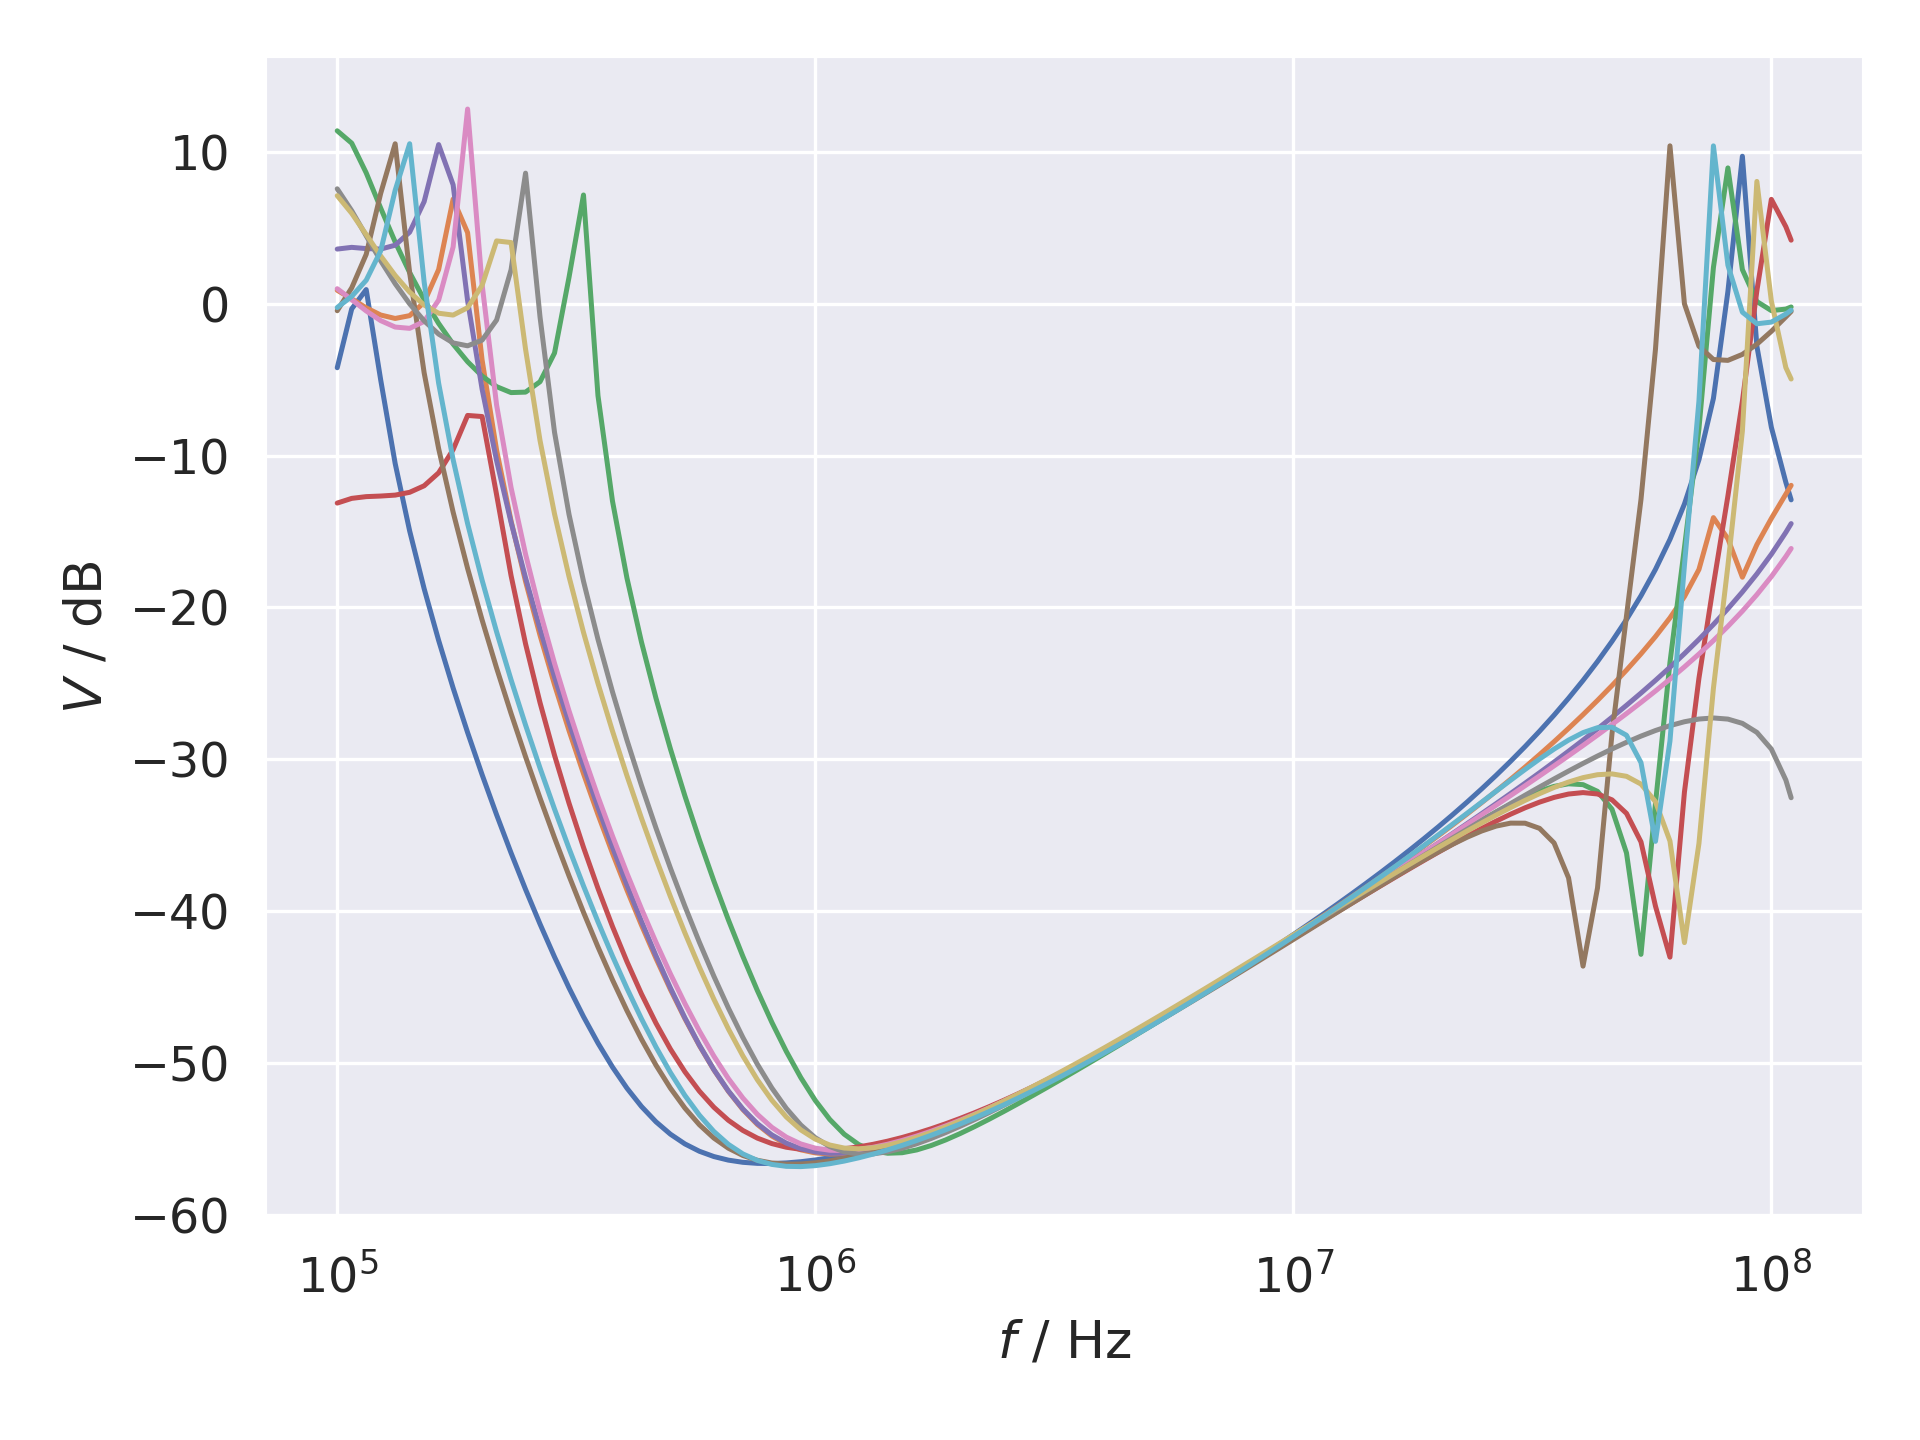
\includegraphics[width=0.6\textwidth]{../plots/data_samples.png}
    \caption{Samples from the training data for frequency domain}
    \label{fig:training_samples}
\end{figure}
\begin{figure}[h]
    \centering
    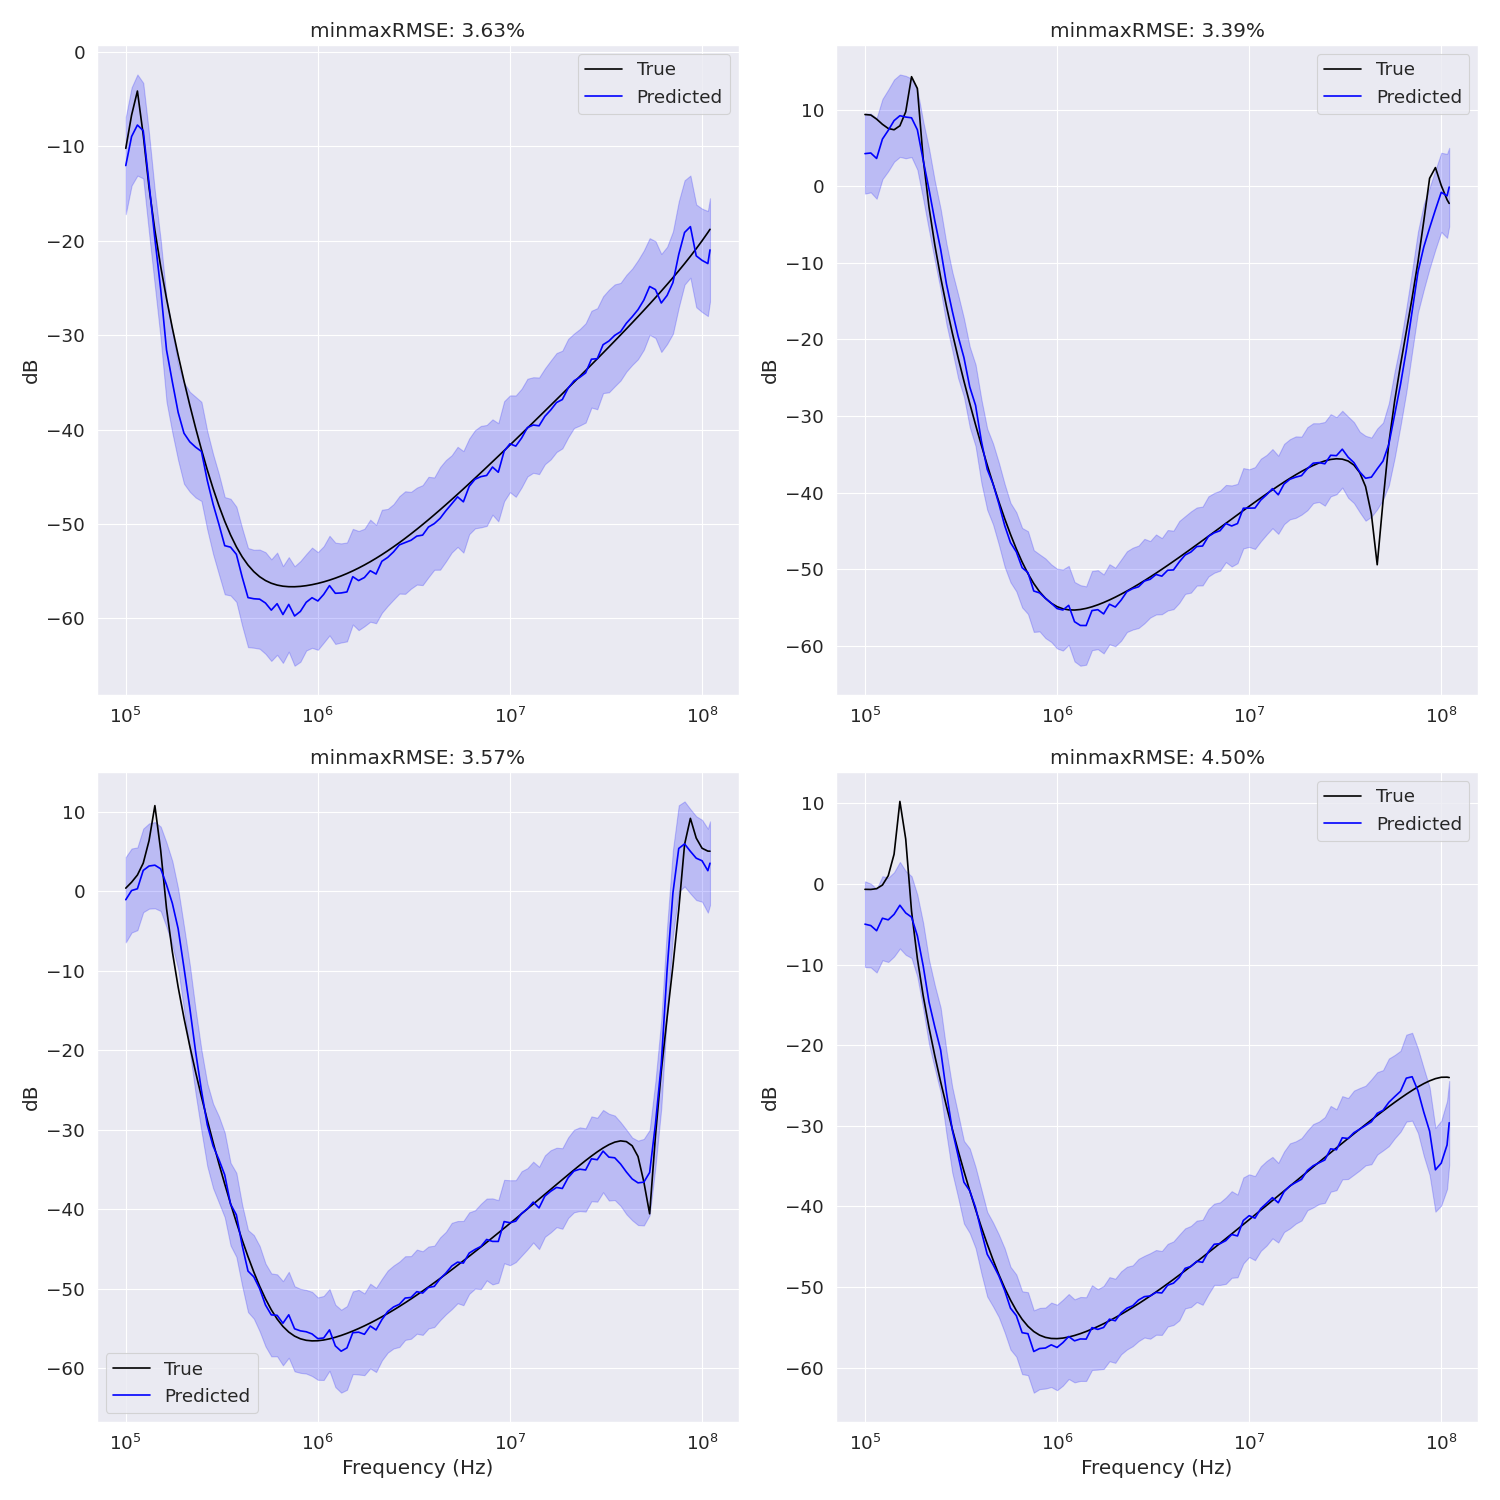
\includegraphics[width=0.6\textwidth]{../plots/prediction_transformer.png}
    \caption{Samples from the training data for frequency domain}
    \label{fig:training_samples}
\end{figure}
\section{Code}
\lstinputlisting[caption={Example Python Code}, label={lst:examplecode}, firstline=10, lastline=30]{../code/transformer_surrogate.ipynb}
\cite{alvarez2012kernels} \cite{raissi2017physicsIDL}

\newpage
\printbibliography

\end{document}